\section{QP2. Erros introduzidos pelos provedores}
\label{sec:qp2:results}

Nesta Seção estão os resultados e a análise dos dados relacionados à segunda questão de pesquisa: ``Como os pacotes provedores introduzem \textit{breaking changes} em uma \textit{release}?''.

\subsubsection{Descoberta \#5: Categorias de \textit{Breaking changes}}

Ao todo, foram descobertos 64 casos de \textit{breaking changes} distribuídas em 45 clientes. Todos esses casos foram agrupados em 8 categorias das quais se combinavam os casos semelhantes. A Tabela \ref{tab:bc_category} apresenta cada uma dessas categorias, bem como a quantidade de pacotes e a quantidade de \textit{releases} que cada categoria impactou.

\begin{table*}\centering
	\begin{tabular}{lrrrrr} \toprule
		\textbf{Categoria} & \multicolumn{2}{c}{\textbf{Casos}} & \phantom{ab} & \multicolumn{2}{c}{\textit{\textbf{Releases}}}
		\\
		\cmidrule{2-3} \cmidrule{5-6}
		& (\#) & (\%) && (\#) & (\%) \\ \midrule
		Alteração de funcionalidade  & 25              & 39,06 && 101                         & 22,44 \\
		Provedores incompatíveis     & 15              & 23,44 && 64                          & 14,22 \\
		Alteração de tipo de objeto  & 9               & 14,06 && 213                         & 47,33 \\
		Objeto indefinido            & 5               & 7,81  && 28                          & 6,22 \\
		Código incorreto             & 5               & 7,81  && 14                          & 3,11  \\
		Código desatualizado         & 2               & 3,13  && 24                          & 5,33 \\
		Renomeação de função         & 2               & 3,13  && 2                           & 0,44  \\
		Arquivo não encontrado       & 1               & 1,56  && 4                           & 0,89  \\ \hline
		\textbf{Total}               & \textbf{64}     &       && \textbf{450}              &       \\
		\bottomrule
	\end{tabular}
    \caption{Categorias dos casos de \textit{breaking changes}}
    \label{tab:bc_category}
\end{table*}

A seguir, encontra-se uma descrição sobre cada categoria e um exemplo que foi encontrado na análise manual sobre como os provedores introduziram um erro em cada categoria.

\begin{itemize}
    \item \textbf{Alteração de funcionalidade}: os casos dessa categoria foram os que mais impactaram os clientes. Essa categoria contém os casos de \textit{breaking change} no qual os provedores possuíam um determinado comportamento, mas alteraram algumas de suas regras/funcionalidades e impactaram os seus clientes. Não foi uma simples alteração no código, mas sim uma alteração em regras no qual os clientes tinham como sólida. Por exemplo, a \textit{release} \textsf{request@2.17.0} -- essa \textit{release} foi removida do \textsf{npm}, mas a alteração se manteve -- introduziu uma alteração em seu código,\footnote{https://github.com/request/request/commit/d05b6ba} como pode ser visto no Código \ref{diff:bc_category_change_rule_1}.

    \begin{lstlisting}[numbers=none, language=diff, label=diff:bc_category_change_rule_1, caption={Exemplo da categoria \textit{Alteração de funcionalidade}}]
  debug('emitting complete', self.uri.href)
+ if(response.body == undefined && !self._json) {
+   response.body = "";
+ }
  self.emit('complete', response, response.body)
    \end{lstlisting}

    Nesse caso, o \textsf{request} adiciona uma \textit{string} vazia ao invés de manter \textit{undefined} no corpo de uma requisição. Esse caso do \textsf{request} ocorreu porque os pacotes provedores evoluem independentemente dos clientes \cite{Foo:2018:ESC:3236024.3275535}. Essa alteração na regra do \textsf{request} reflete em uma evolução do pacote, mas os clientes não esperavam essa alteração e confiavam que o corpo da resposta fosse retornado como \textit{undefined}, por isso os clientes sofreram um erro.

    \item \textbf{Provedores incompatíveis}: nessa categoria, há um provedor direto \textsf{A} e um provedor indireto \textsf{B} envolvido, o qual alterou o seu código, o que não gerou um erro, mas provocou um comportamento inesperado no provedor \textsf{A}. Ou seja, o provedor \textsf{B} passou a ser incompatível com o provedor \textsf{A}. Nessa categoria, nenhum dos provedores contém um erro, mas sim uma incompatibilidade. Um exemplo disso ocorreu com os pacotes \textsf{babel-eslint} e \textsf{escope}, sendo o pacote \textsf{escope} é um provedor indireto do \textsf{babel-eslint}.

    \begin{lstlisting}[numbers=none, language=diff, label=cod:bc_category_incompatibles_providers, caption={Exemplo da categoria \textit{Provedores incompatíveis}}]
  }
-   },
-   visitClass: {
+ }, {
+   key: 'visitClass',
        value: function visitClass(node) {
    \end{lstlisting}

    A \textit{release} \textsf{escope@3.4} realizou uma alteração no seu código, conforme o Código \ref{cod:bc_category_incompatibles_providers}, mas que não reflete em um erro. Essa alteração impactou diretamente o pacote \textsf{babel-eslint}, mesmo o pacote \textsf{escope} não sendo um provedor direto do \textsf{babel-eslint} e não ter introduzido um erro.\footnote{https://github.com/estools/escope/issues/99\#issuecomment-178151491} Com isso, houve uma incompatibilidade entre os provedores e essa incompatibilidade precisou ser corrigida pelo \textsf{babel-eslint}. Essa \textit{breaking change} manteve-se não-consertada por apenas um dia, mas durante esse período o \textsf{babel-eslint} foi descarregado \textit{80k} vezes do \textsf{npm}.

    \item \textbf{Alteração de tipo de objeto}: em linguagens fortemente tipadas essa categoria de \textit{breaking change} não ocorre, mas no \textsf{Javascript} representam um tipo de \textit{breaking change} que, por muitas vezes, pode nem se manifestar no cliente. Mas, neste trabalho, foram detectados 9 (14.06\%) casos nos quais os provedores alteraram o tipo de algum objeto.

    \begin{lstlisting}[numbers=none, language=diff, label=cod:bc_category_change_type, caption={Exemplo da categoria \textit{Alteração de tipo de objeto}}]
  this.setup();
- this.sockets = [];
+ this.sockets = {};
  this.nsps = {};
    this.connect Buffer = [];
  }
  var socket = nsp.add(this, function() {
-   self.sockets.push(socket);
+   self.sockets[socket.id] = socket;
    self.nsps[nsp.name] = socket;
    \end{lstlisting}

    No Código \ref{cod:bc_category_change_type} o provedor \textsf{socket.io} alterou um \textit{array} para \textit{object}.\footnote{https://github.com/socketio/socket.io/commit/b73d9be} Anteriormente, os clientes iteravam nesse \textit{array}, mas após essa alteração os clientes foram impactados por uma \textit{breaking change}. Mesmo sendo uma simples alteração, muitos clientes do \textsf{socket.io} foram impactados, até mesmo o pacote \textsf{karma},\footnote{https://github.com/socketio/socket.io/issues/2368} um utilitário para testes em \textit{browsers}, que foi forçado a alterar seu código\footnote{https://github.com/karma-runner/karma/commit/3ab78d6} e publicar a \textit{relese} \textsf{karma@0.13.19}. Enquanto essa \textit{breaking change} manteve-se não-resolvida por apenas um dia, o \textsf{karma} recebeu \textit{146k downloads} do \textsf{npm}.

    \item \textbf{Objeto indefinido}: por vezes, os códigos podem estar todos corretos, mas então os provedores tentam acessar uma variável que não existe. Esta categoria de \textit{breaking change} representa os casos no qual os provedores tentaram obter acesso à alguma variável/objeto, mas que não existiam.

    \begin{lstlisting}[numbers=none, language=diff, label=cod:bc_category_undefined_object, caption={Exemplo da categoria de \textit{Objeto Indefinido}}]
+ app.options = app.options || {};
  app.options.babel = app.options.babel || {};
  app.options.babel.plugins = app.options.babel.plugins || [];
    \end{lstlisting}

    Esse tipo de erro surgiu na \textit{release} \textsf{ember-cli-htmlbars-inline-precompile@0.1.3}, na qual o desenvolvedor tenta acessar uma variável que não estava disponível. Mas, assim como o desenvolvedor já havia feito com as demais variáveis do Código \ref{cod:bc_category_undefined_object}, uma simples alteração no código\footnote{https://github.com/ember-cli/ember-cli-htmlbars-inline-precompile/pull/5/commits/b3faf959} foi o suficiente.

    \item \textbf{Código incorreto}: este caso de \textit{breaking change} ocorreu quando os provedores escreveem um código semanticamente incorreto, gerando um erro na sua execução e afetando os clientes. Em linguagens compiladas, esse tipo de erro seria facilmente identificado em tempo de compilação, mas no \textsf{Javascript} esse tipo de erro apenas se manifesta em tempo de execução. Foi o que ocorreu com a \textit{release} \textsf{front-matter@0.2.0}.

	 \begin{lstlisting}[numbers=none, language=diff, label=cod:bc_category_wrong_code, caption={Exemplo da categoria \textit{Código incorreto}}]
  const separators = [ '---', '= yaml =']
- const pattern = pattern = '^('
+ const pattern = '^('
    + '((= yaml =)|(---))'
	 \end{lstlisting}

    Apesar de ser um erro facilmente detectável e corrigível, como o provedor fez\footnote{https://github.com/jxson/front-matter/commit/f16fc01} no Código \ref{cod:bc_category_wrong_code}, o provedor \textsf{front-matter} aguardou aproximadamente um ano para corrigir e publicar a \textit{release} \textsf{front-matter@0.2.2}. Durante esse período, \textsf{front-matter} foi descarregado do \textsf{npm} 366 vezes.

    \item \textbf{Código desatualizado}: nessa categoria um provedor \textsf{A} atualiza o seu provedor \textsf{B} explicitamente -- alterando manualmente o \textit{range} do seu provedor no \textit{package.json} --, mas o provedor \textsf{A} não atualiza o seu código para executar de acordo com a nova versão do provedor \textsf{B}. Então, uma \textit{breaking change} é introduzida nos pacotes clientes. Além de um caso de atualização explícita, foi detectado um caso no qual um provedor \textsf{A} especificou um provedor \textsf{B} com o \textit{X-range ($>$=)}, e ao longo do tempo o provedor \textsf{B} publicou uma \textit{release major} que introduziu \textit{breaking changes}. Apesar do provedor \textsf{A} especificar um \textit{X-range}, \textsf{A} não atentou-se para a atualização implícita de \textsf{B} com uma \textit{breaking change}, e essa \textit{breaking change} foi cascateada para os clientes.

    \item \textbf{Renomeação de função}: as \textit{breaking changes} relacionadas à esta categoria são facilmente detectáveis. Quando a mensagem de erro do \textsf{Node.js} é exibida como \textit{TypeError: var is not a function}, provavelmente trata-se de uma determinada função que não esta disponível, ou seja, foi removida ou renomeada. Todas os dois casos nesta categoria ocorreram porque a função foi renomeada. O primeiro caso está descrito nos exemplos motivacionais (Capítulo \ref{cap:exemplos}).

	 \begin{lstlisting}[numbers=none, language=diff, label=cod:bc_category_renamed_function, caption={Exemplo da categoria \textit{Renomeação de função}}]
- RedisClient.prototype.send_command = function (command, args, callback) {
-     var args_copy, arg, prefix_keys;
+ RedisClient.prototype.internal_send_command = function (command, args, callback) {
+     var arg, prefix_keys;
	 \end{lstlisting}

    O segundo caso ocorreu quando a \textit{release} \textsf{redis@2.6.0-1} renomeou uma função, como no Código \ref{cod:bc_category_renamed_function}.\footnote{https://github.com/NodeRedis/node\_redis/commit/861749f} Entretanto, essa função era apenas utilizada internamente pelo pacote \textsf{fakeredis},\footnote{https://github.com/NodeRedis/node-redis/issues/1030\#issuecomment-205379483} que foi impactado pela \textit{breaking change}. Essa \textit{breaking change} foi corrigida no pacote cliente \textsf{fakeredis@1.0.3} que realizou um \textit{downgrade} para a versão \textsf{redis@2.6.0-0}.\footnote{https://github.com/hdachev/fakeredis/commit/01d1e99} Em cinco dias dos quais a \textit{breaking change} não foi corrigida, o \textsf{fakeredis} foi descarregado \textit{2.3k} vezes do \textsf{npm}.

    \item \textbf{Arquivo não encontrado}: os casos de \textit{breaking change} relacionados à esta categoria são aqueles no qual os desenvolvedores realizam um acesso a um arquivo, mas esse não existe. O arquivo requerido pode não existir ou não estar disponível, uma vez que, referenciado no arquivo \textit{.npmignore} -- arquivo utilizado pelo \textsf{npm} para ignorar arquivos durante o processo de publicação --, o arquivo existe mas não está disponível. Entretanto, o único caso de \textit{breaking change} dessa categoria ocorreu pois o provedor referenciou o \textit{index.js} ao \textit{.npmignore}.
\end{itemize}{}

\subsubsection{Descoberta \#6: Nível do Versionamento Semântico que as \textit{breaking changes} são introduzidas}

De todos os 64 casos de \textit{breaking changes}, 3 casos foram introduzidos no nível \textit{major}; 26 casos, no \textit{minor}; 28 casos, no \textit{patch}; e 5 casos, pré-\textit{releases}, como pode ser visto na Tabela \ref{tab:semver_levels}. Apenas foram analisados os casos de \textit{breaking changes} em \textit{releases minor} e \textit{patch}, mas houveram 3 casos em que a \textit{breaking change} foi introduzida em uma \textit{release major}: em dois casos os provedores escreveram códigos errôneos na \textit{release major} e o cliente a estava usando -- como no caso do \textsf{jsdom@16} (Cap. \ref{cap:exemplos}) -- e o terceiro caso ocorreu quando um provedor \textsf{A}, que depende de um provedor \textsf{B}, aceitou a \textit{release} com \textit{breaking change} através do \textit{X-range ($>$=)} do provedor \textsf{B}, mas não tratou essa \textit{breaking change}.

\begin{table}
	\centering
	\caption{Porcentagem de \textit{breaking change} introduzida em cada nível do Versionamento Semântico}
	\begin{tabular}{lrr}
		\toprule
		\textbf{Níveis} & \textbf{(\#)} & \textbf{(\%)} \\ \hline
		\textit{Major}       & 03       & 4.69          \\
		\textit{Minor}       & 28       & 43.75         \\
		\textit{Patch}       & 28       & 43.75         \\
		Pré\textit{-release} & 05       & 7.8           \\ \bottomrule
	\end{tabular}
	\label{tab:semver_levels}
\end{table}

Pré-\textit{releases} antecedem suas \textit{releases} estáveis, mas não são consideradas estáveis; qualquer alteração não-retro compatível deve ser resolvida até a versão estável ser publicada.\footnote{https://semver.org/\#spec-item-9} Foi detectado \textit{breaking changes} em 5 casos de pré-\textit{releases}, mas esses provedores cascatearam essas \textit{breaking changes} para as \textit{releases} estáveis. Por exemplo, a pré-\textit{release} \textsf{redis@2.6.0-1}, descrita na categoria \textit{Renomeação de função} da Seção \ref{sec:qp2:results}, alterou o nome de uma função, e essa alteração não-retro compatível deveria ser corrigida até a \textit{release} estável \textsf{redis@2.6.0}, mas essa alteração foi propagada para a \textit{release} estável, impactando e execução do cliente com uma \textit{breaking change}. Esse exemplo mostra como os provedores não estão devidamente orientados sobre as regras do Versionamento Semântico.

\subsubsection{Descoberta \#7: Provedores introduzem a mesma quantidade de \textit{breaking changes} em \textit{releases minor} e \textit{patch}}

Os provedores introduzem \textit{breaking changes} em níveis não-\textit{major} em dois cenários: 1) em \textit{releases minor}, quando os provedores tinha a intenção de publicar novas funcionalidades retro-compatíveis, mas essas funcionalidades tornaram-se \textit{breaking changes}; e 2) em \textit{releases patch}, quando os provedores tinha o propósito de publicar correções de erros. Nos casos das \textit{releases patch}, os provedores estavam realmente tentando publicar uma correção de erro, mas essas alterações podem não ter consertado o erro anterior, mas sim introduzido mais erros. Para casos em \textit{releases minor}, essas novas funcionalidades podem ser casos reais de \textit{breaking changes} dos quais os provedores têm a responsabilidade de corrigir, ou podem ser novas funcionalidades que os clientes precisam se adaptar. Para analisar esse impasse, foi observado qual pacote corrigiu a \textit{breaking change} e para qual nível a nova \textit{release} foi publicada. A Figura \ref{fig:semver_fixed} apresenta esses dados.

\begin{figure}
	\centering
	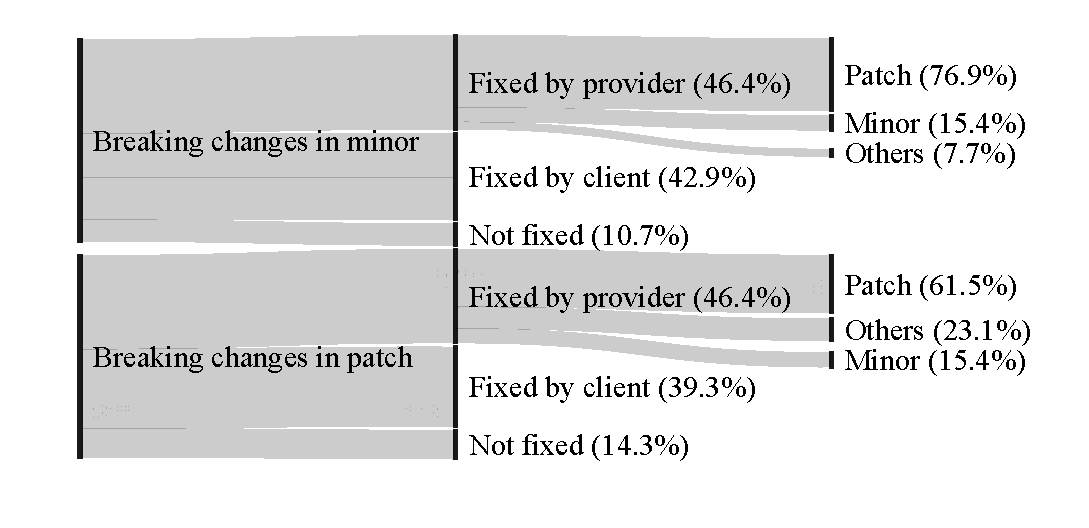
\includegraphics[scale=0.8]{figuras/semver_fixed_prov.pdf}
	\caption{As \textit{breaking changes} corrigidas pelos pacotes providores e clientes e o respectivo nível do Versionamento Semântico que a \textit{release} de correção foi publicada}
	\label{fig:semver_fixed}
\end{figure}{}

A Figura \ref{fig:semver_fixed} mostra que metade das \textit{breaking changes} introduzidas em \textit{releases minor} são corrigidas pelos pacotes clientes. Ou seja, os provedores introduziram uma funcionalidade retro-compatível que tornou-se uma \textit{breaking change}, mas foram os pacotes clientes quem precisaram se adaptar. Mas, quando os provedores corrigem as \textit{breaking changes} introduzidas em \textit{releases minor}, em 76.9\% dos casos a correção é publicada em uma \textit{release patch} e, de acordo com o Versionamento Semântico, essa \textit{release} tinha a finalidade de corrigir um erro. Portanto, os provedores assumem que, de fato, uma \textit{breaking change} foi introduzida e são eles os responsáveis pela correção.

\textit{Breaking changes} introduzidas em \textit{releases patch} deveriam conter apenas correções de erros, mas os provedores introduziram \textit{breaking changes}. Essas \textit{breaking changes} em \textit{releases patch} são corrigidas pelos provedores em 46.4\% das vezes. Ainda, em 61.5\% das vezes os provedores publicam a correção em uma \textit{release patch}, significando que houve a tentativa de corrigir algo.

\subsubsection{Descoberta \#8: 78.1\% das \textit{breaking changes} possuem pelo menos uma documentação}

Quando uma \textit{breaking change} se manifesta nos pacotes clientes, ela deve ser documentada em \textit{issues} ou \textit{pull-requests}. Essas funcionalidades integradas aos repositórios dos pacotes permitem aos clientes notificarem os provedores sobre erros ou questões acerca do próprio provedor. Também, as \textit{breaking changes} podem ser documentadas em \textit{changelogs}, tanto quando a \textit{breaking change} é introduzida ou quando a mesma é corrigida. As \textit{changelogs} criadas pelos provedores contêm os detalhes das alterações que os provedores introduzem em uma determinada \textit{release}.

\begin{table}
	\centering
	\caption{Como cada \textit{breaking change} foi documentada}
	\begin{tabular}{lrr}
		\toprule
		\textbf{Documentação} & \textbf{(\#)} & \textbf{(\%)}   \\ \hline
		\textit{Issue}        & 32            & 64              \\
		\textit{Pull-request} & 22            & 44              \\
		\textit{Changelog} de introdução & 23 & 46              \\
		\textit{Changelog} de correção   & 16 & 32              \\ %\midrule
		%\textbf{Total}         & \textbf{50} & \textbf{78.1\%} \\ 
		\bottomrule
	\end{tabular}
	\label{tab:bc_documentation}
\end{table}

A Tabela \ref{tab:bc_documentation} mostra que as \textit{breaking changes} são documentadas em 55 (78.1\%) casos. Dos casos documentados, 70\% possuem mais de um tipo de documentação. Por exemplo, o provedor foi notificado de uma \textit{breaking change} através de uma \textit{issue}, corrigiu-a e a documentou em seu \textit{changelog}. Nesse caso houveram duas documentações. Esse é um número positivo para os clientes, uma vez que quando a mesma \textit{breaking change} se manifesta em vários clientes, mas já foi previamente documentada, torna-se fácil para os clientes se recuperarem. Por fim, em 14 (21.9\%) casos a \textit{breaking change} não foi documentada.

\begin{mdframed}
Destaques da QP2: Os defeitos mais comuns nos pacotes provedores que causam \textit{breaking changes} são aqueles relacionados com uma alteração de funcionalidade, quando dois provedores se tornam incompatíveis e alterações nos tipos de objetos. Os provedores introduzem \textit{breaking changes} em níveis \textit{minor} e \textit{patch} na mesma frequência. A maioria das \textit{breaking changes} corrigidas pelos provedores são publicada em \textit{releases patch}. As \textit{breaking changes} são documentadas em 78.1\% dos casos e a principal funcionalidade usada para documentação são as \textit{issues}.
\end{mdframed}